\chapter{Ступенчатое понижение промежуточного представления}\label{ch:lowering}

\section{Физическая модель и типы памяти в GPGPU}\label{sec:lowering/physical}

\begin{figure}[ht]
    \centerfloat{
        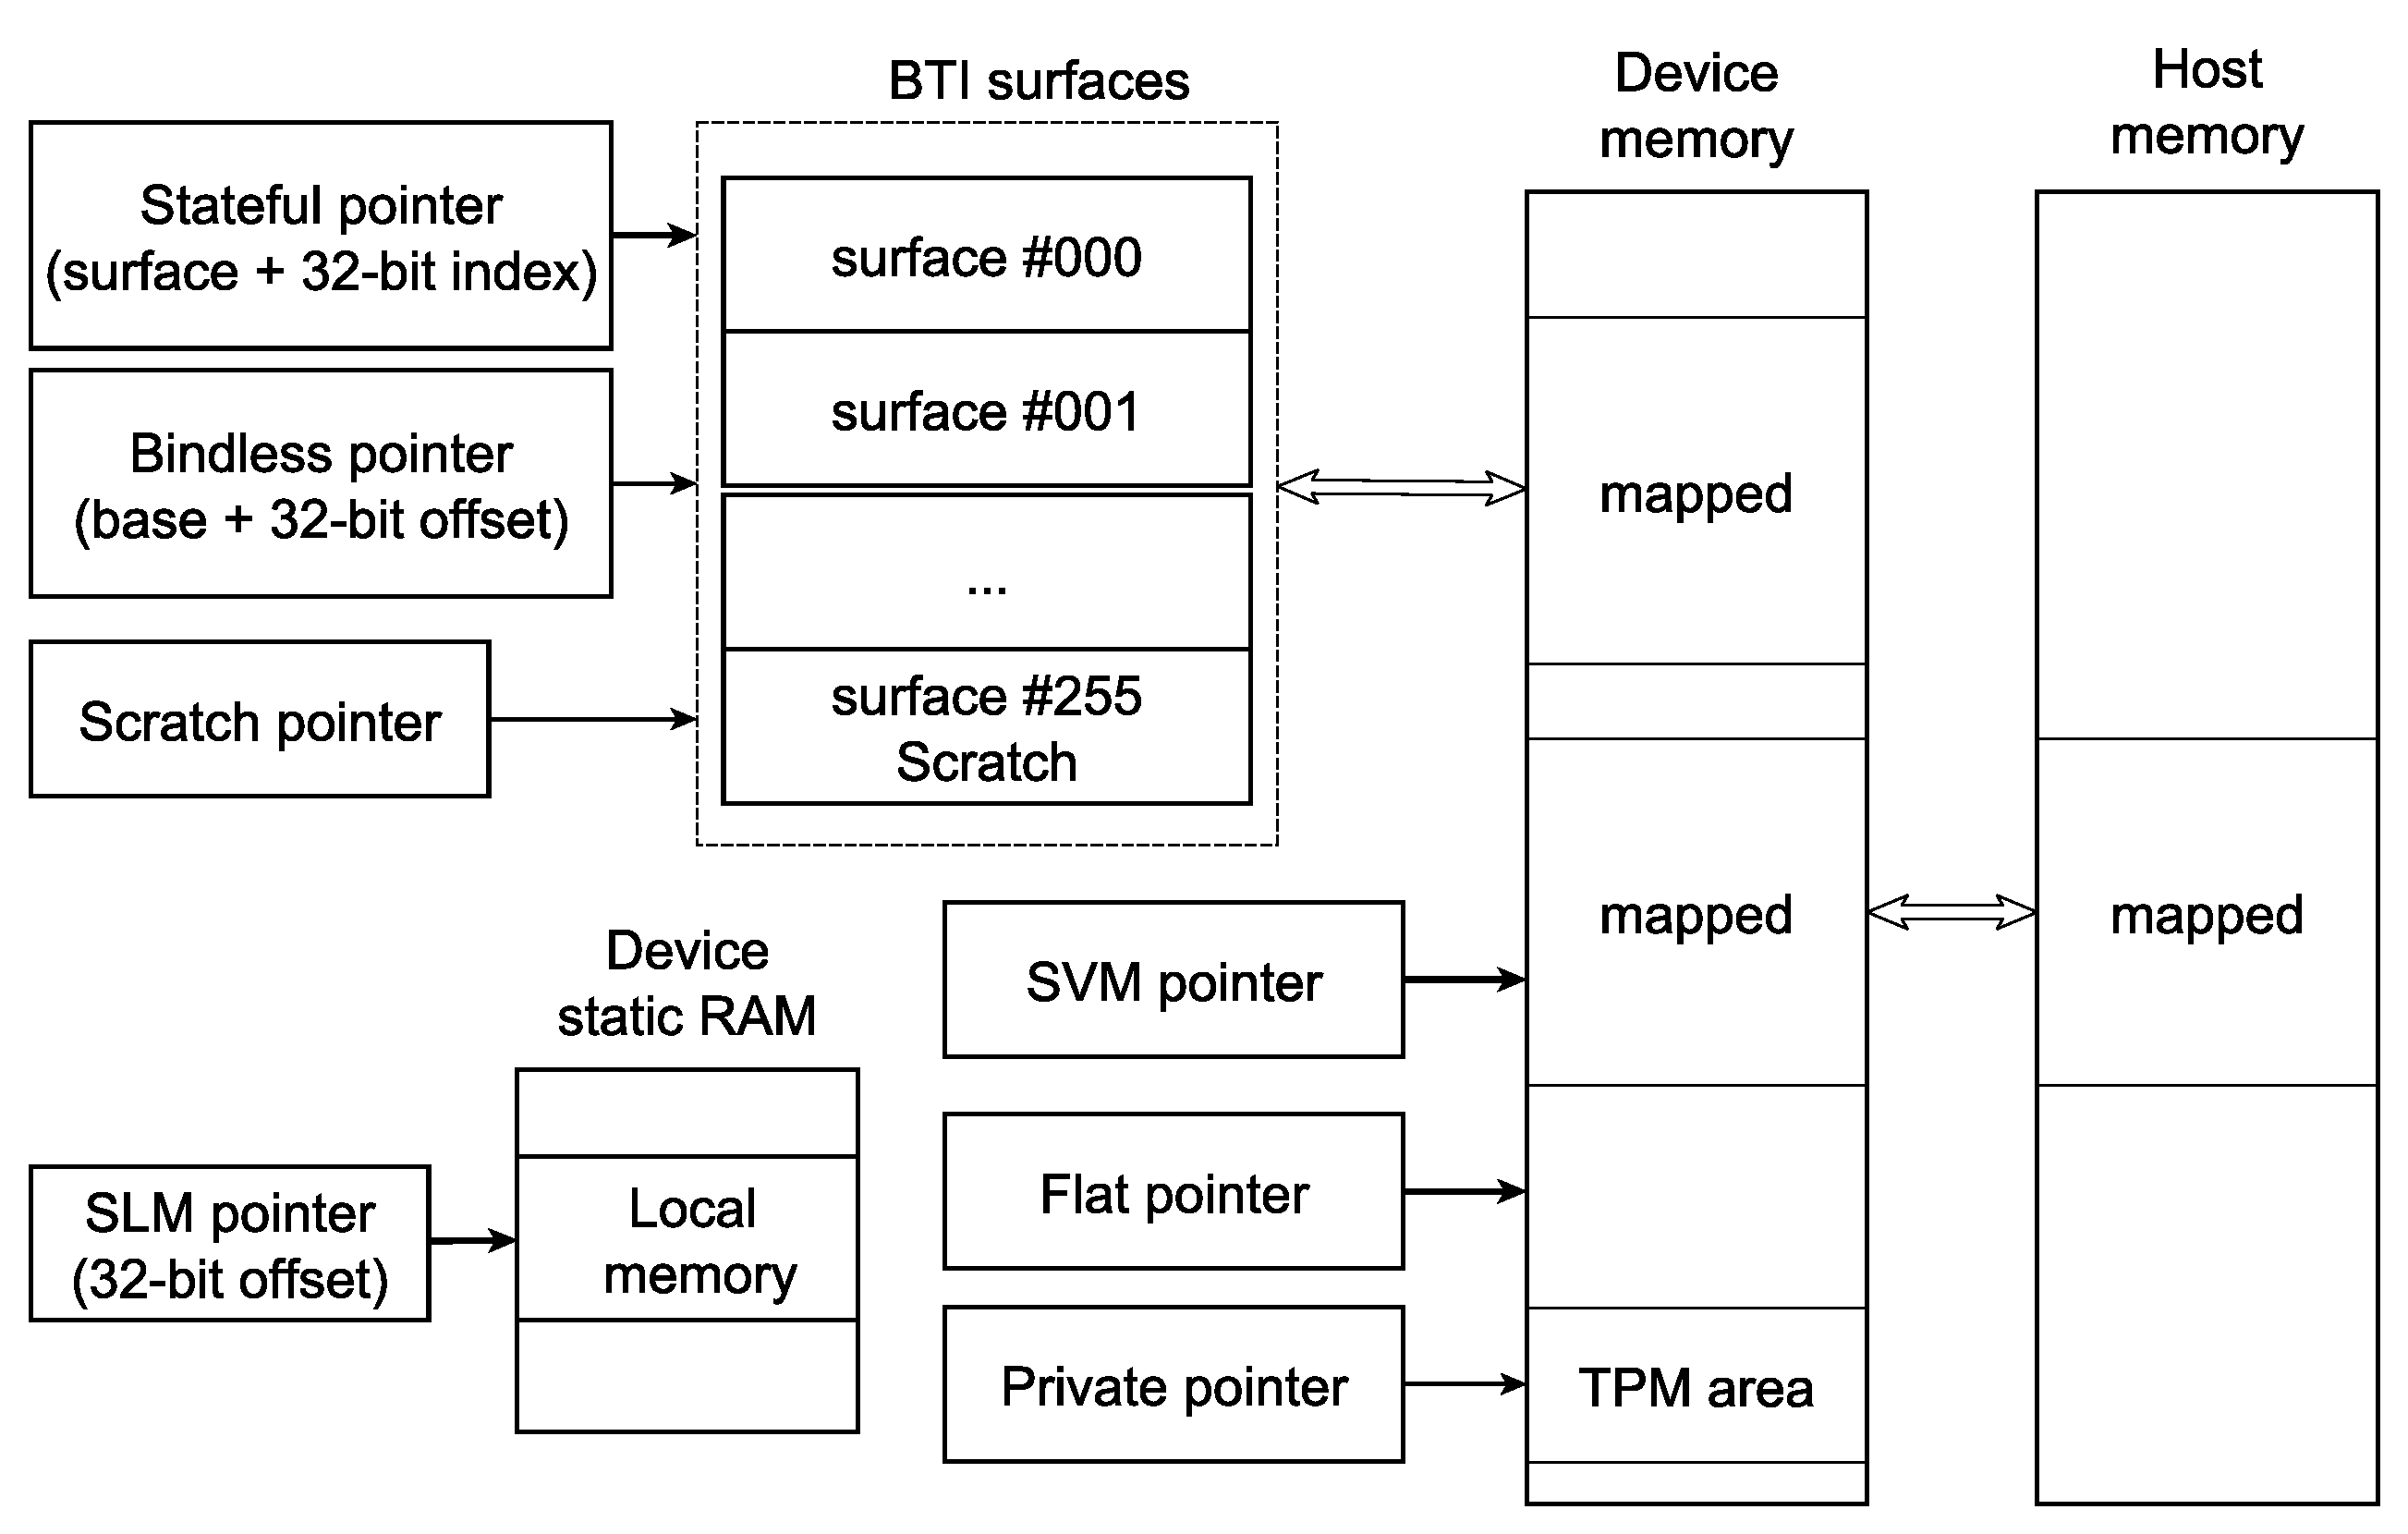
\includegraphics[scale=0.4]{Vladimirov/images/memory-scheme.pdf}
    }
    \caption{Физическая модель памяти}\label{fig:memory-scheme}
\end{figure}

Физическая модель памяти представлена на рисунке~\cref{fig:memory-scheme}

Тут про stateful, stateless, SVM и прочее

\section{Предлагаемые улучшения в pass manager}\label{sec:lowering/passes}

\begin{figure}[ht]
    \centerfloat{
        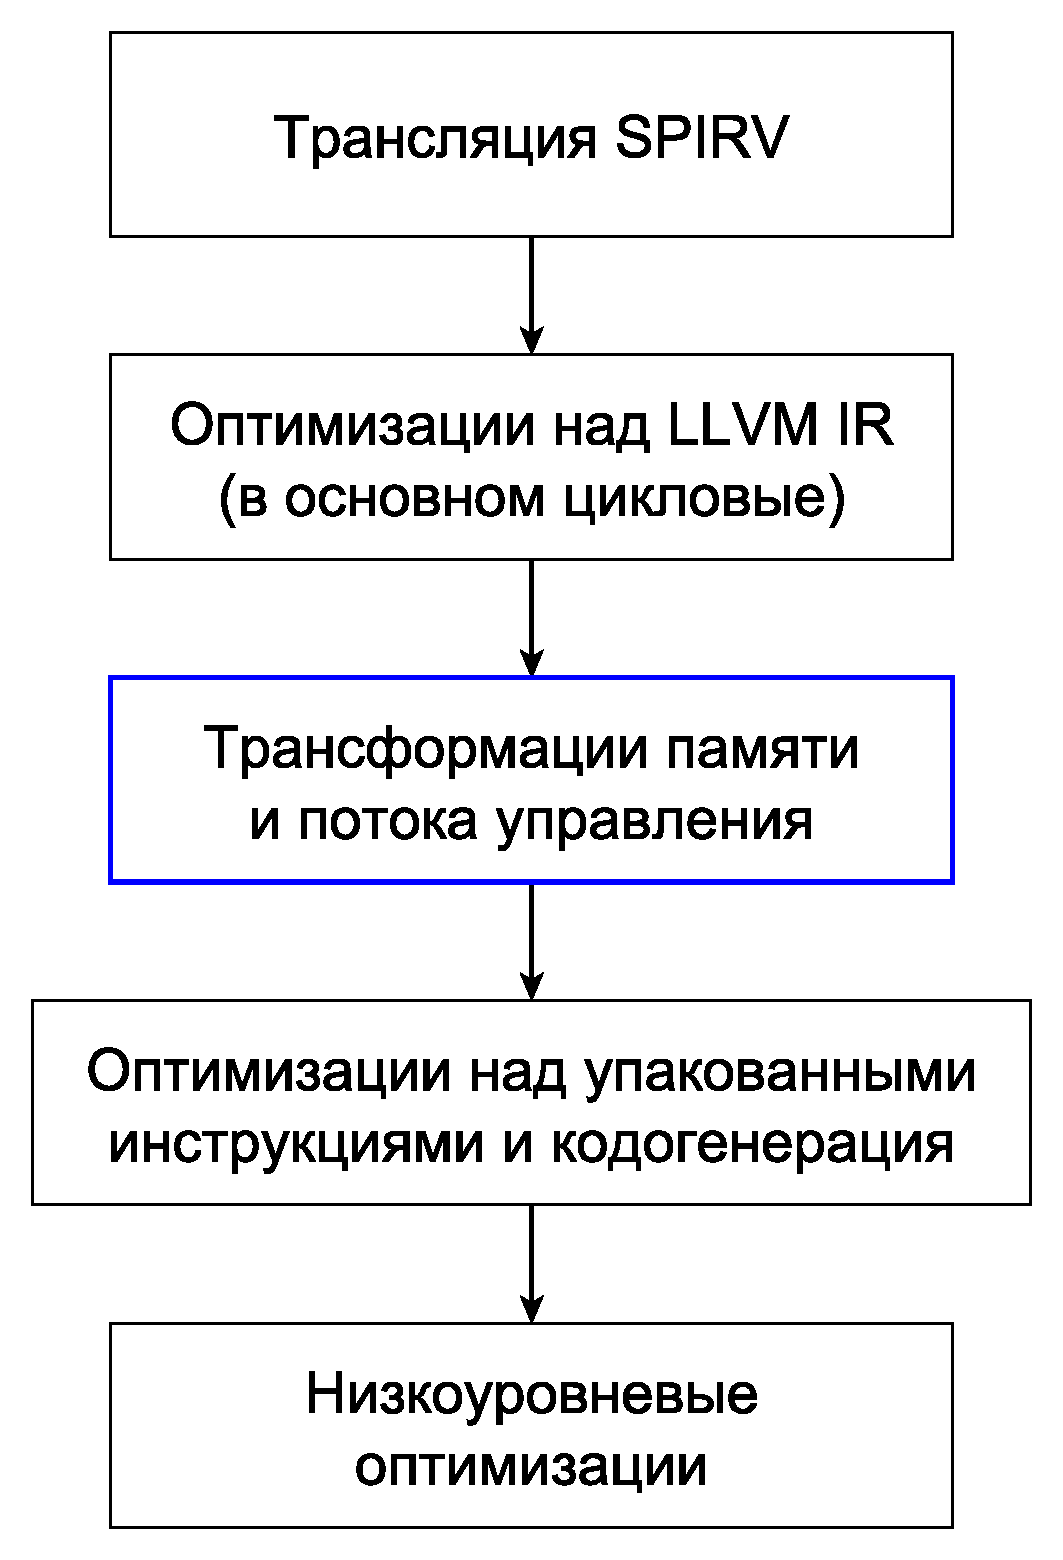
\includegraphics[scale=0.4]{Vladimirov/images/highlevel-mgr.pdf}
    }
    \caption{Высокоуровневый список трансформаций}\label{fig:highlevel-mgr}
\end{figure}

Высокоуровнеая схема менеджера пассов представлена на рисунке~\cref{fig:highlevel-mgr}

\begin{figure}[ht]
    \centerfloat{
        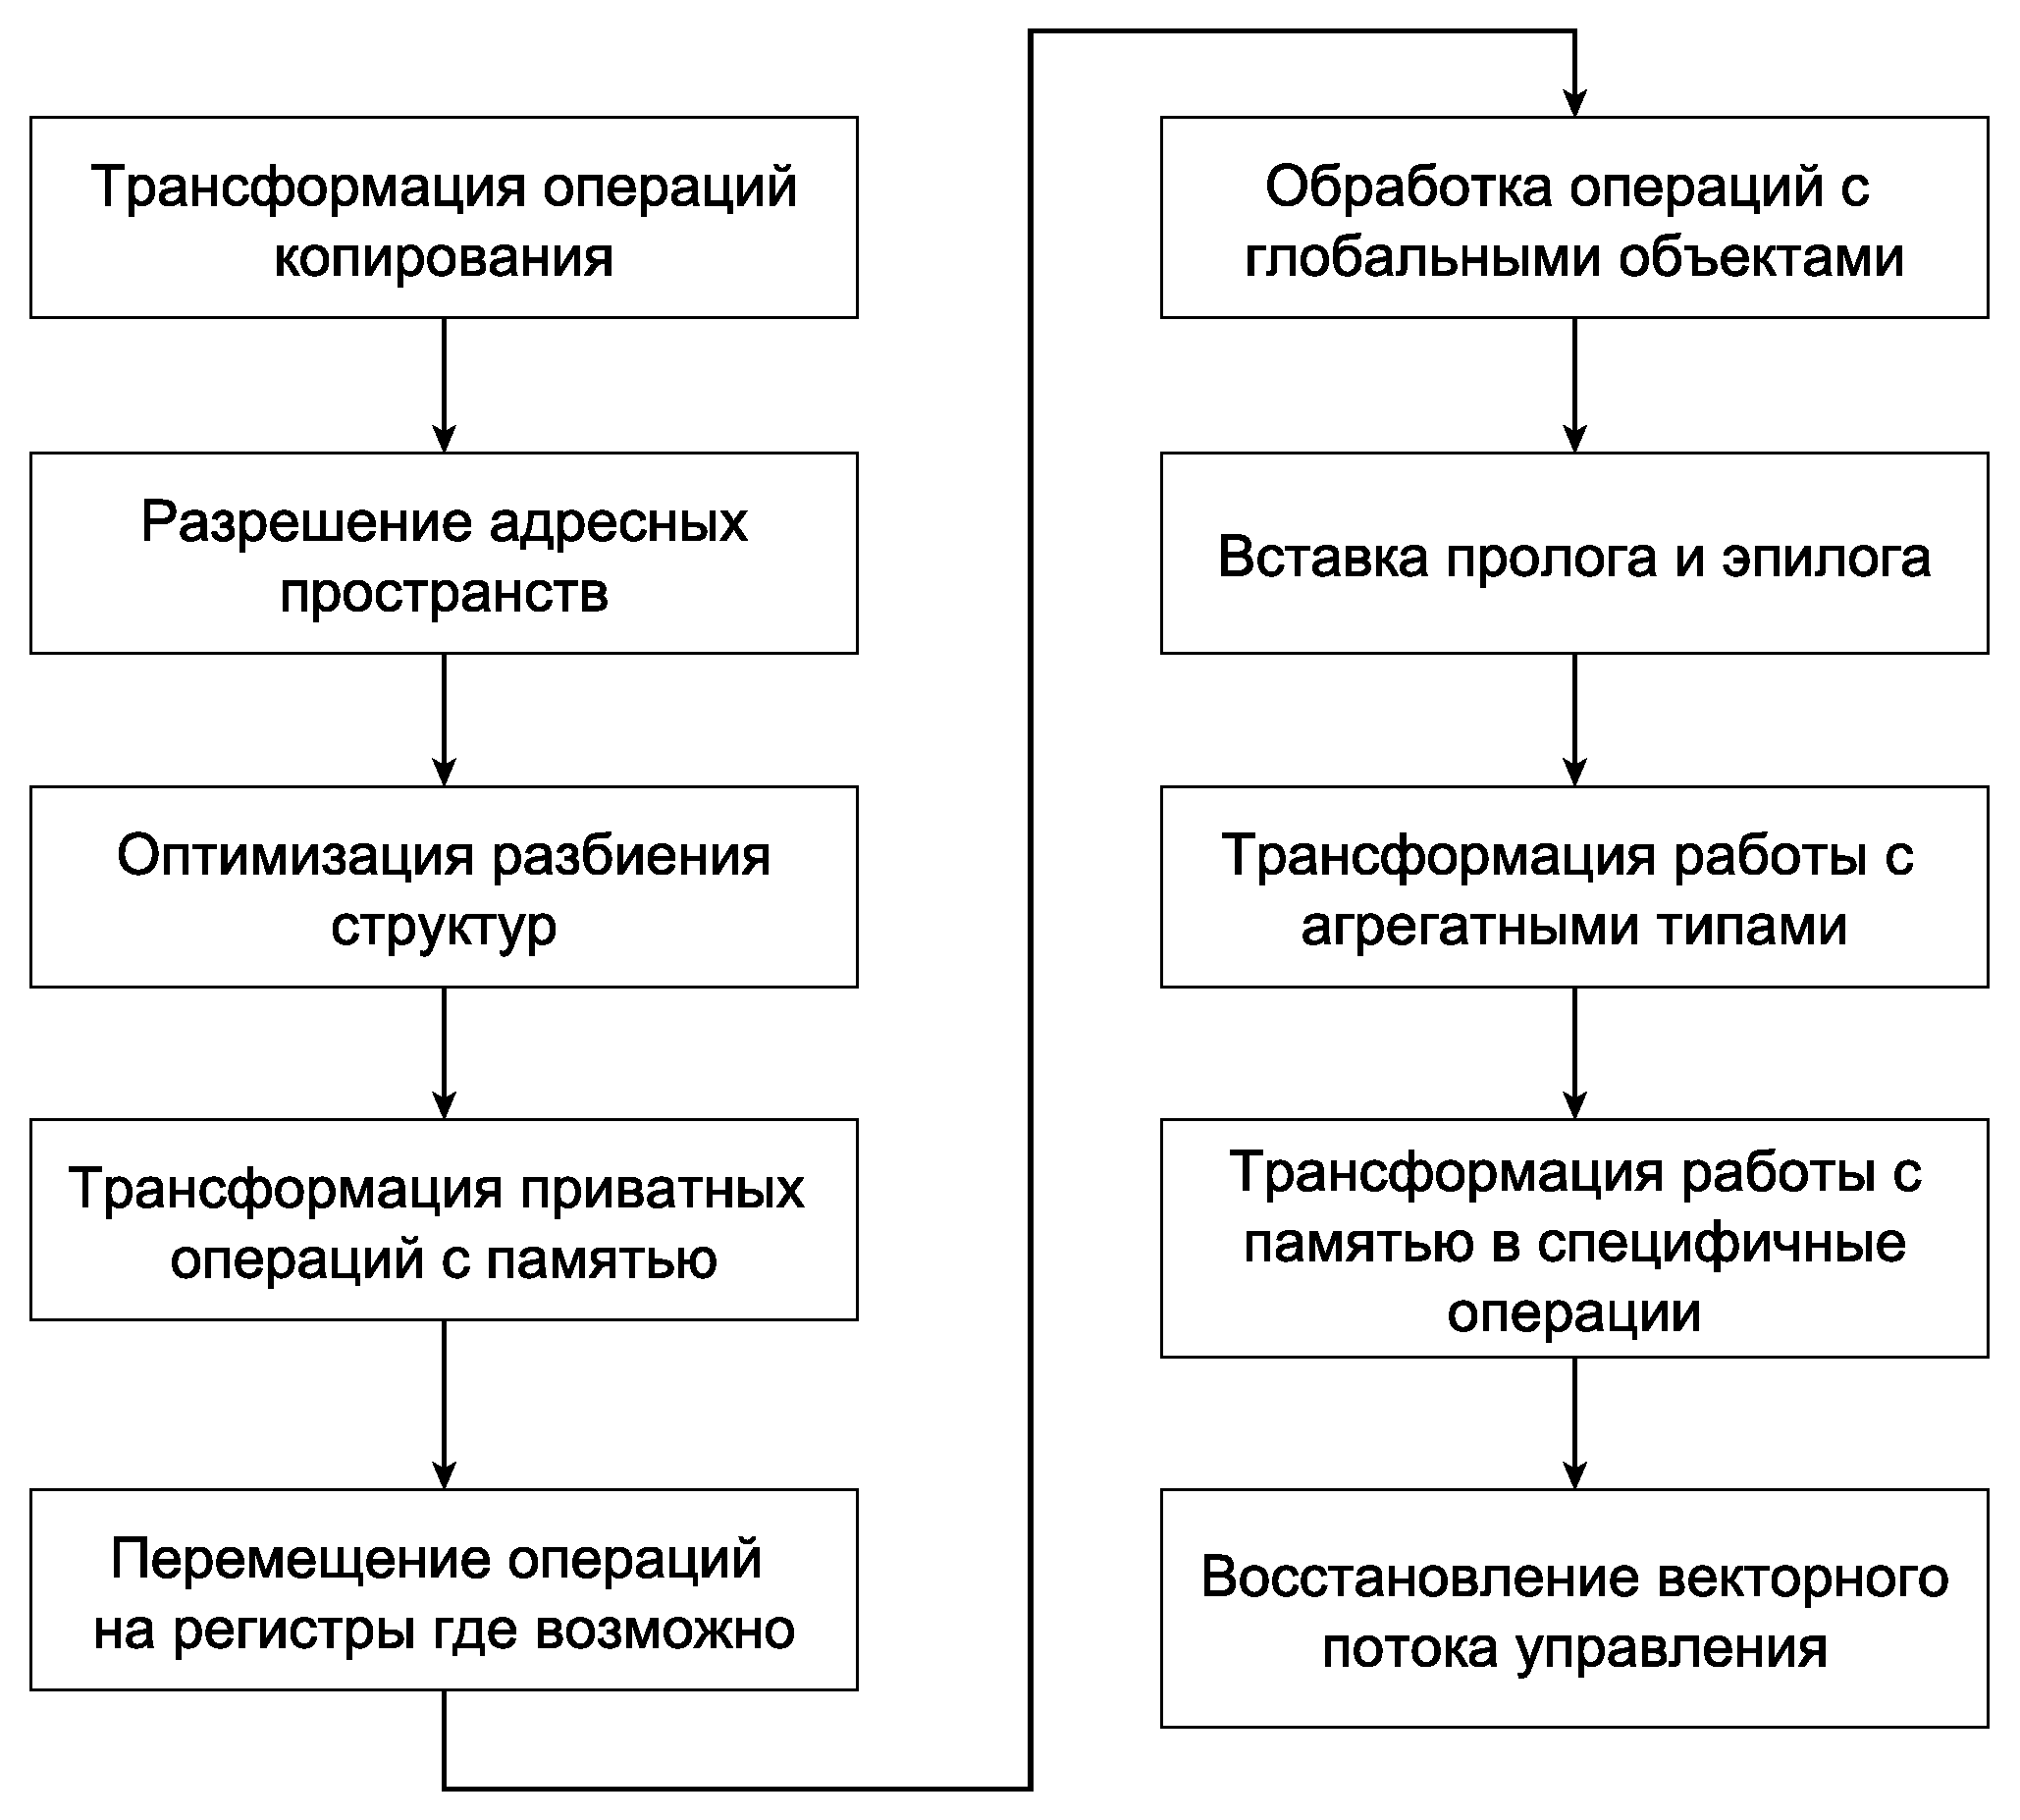
\includegraphics[scale=0.4]{Vladimirov/images/passmgr.pdf}
    }
    \caption{Детальный список трансформаций}\label{fig:passmgr}
\end{figure}

Детальный pass manager представлен на рисунке~\cref{fig:passmgr}

